\documentclass[11pt,letterpaper]{article}
\usepackage[lmargin=1in,rmargin=1in,tmargin=1in,bmargin=1in]{geometry}
\usepackage{../style/homework}
\usepackage{../style/commands}
\setbool{quotetype}{true} % True: Side; False: Under
\setbool{hideans}{true} % Student: True; Instructor: False

% -------------------
% Content
% -------------------
\begin{document}

\homework{18: Due 12/11}{Go down deep enough into anything and you will find Mathematics.}{Dean Schlicter}

% Problem 1
\problem{10} Consider the polynomial $f(x)= (x - 1)(x + 3)(x^2 + 4)(x^2 - 9)$. 
	\begin{enumerate}[(a)]
	\item What is the degree of $f(x)$?
	\item How many real zeros does $f(x)$ have?
	\item How many complex zeros does $f(x)$ have?
	\item Does $f(x)$ have a maximum or a minimum? Explain. 
	\end{enumerate}



\newpage



% Problem 2
\problem{10} Determine the quadratic polynomial that has a root at $x= 1 - 3i$ and has $y$-intercept 5.



\newpage



% Problem 3
\problem{10} Suppose that $f(x)$ is a degree four polynomial (quartic polynomial) with $f(-3)= f(1)= f(4)= f(6)= 0$ and $f(0)= -7$. Find the polynomial $f(x)$. 



\newpage



% Problem 4
\problem{10} Suppose $f(x)$ is a real quartic polynomial whose graph is given below. How many real zeros does $f(x)$ have? How many complex zeros does $f(x)$ have? Find $f(x)$. 
	\[
	\fbox{
	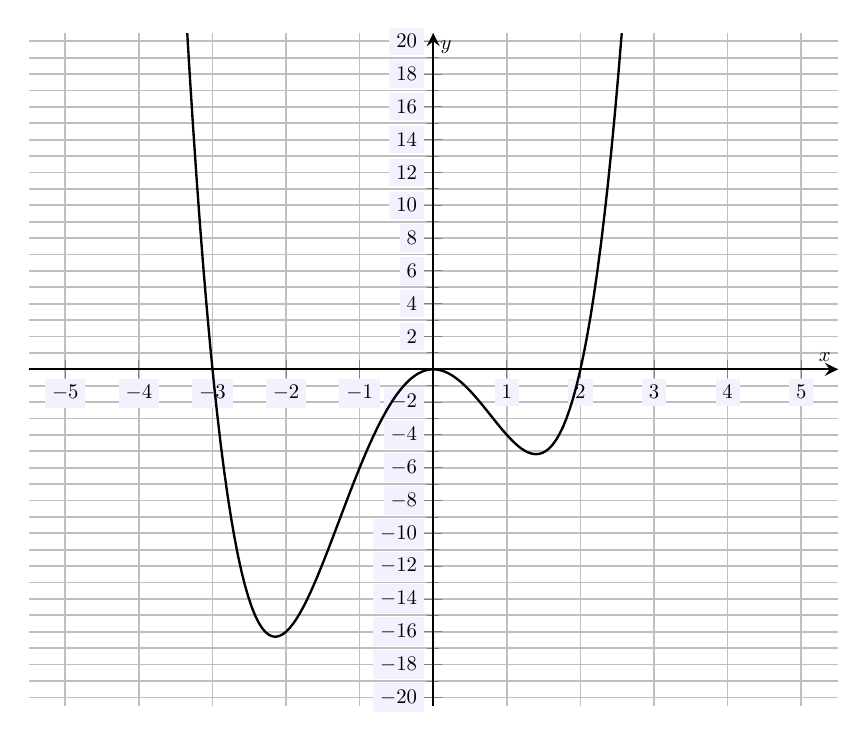
\begin{tikzpicture}[scale=1.5,every node/.style={scale=0.5}]
	\begin{axis}[
	grid=both,
	axis lines=middle,
	ticklabel style={fill=blue!5!white},
	xmin= -5.5, xmax=5.5,
	ymin= -20.5, ymax=20.5,
	xtick={-5,-4,...,5},
	ytick={-20,-18,...,20},
	minor tick = {-20,-19,...,20},
	xlabel=\(x\),ylabel=\(y\),
	]
	\addplot[line width= 0.02cm,samples=150,domain= -3.5:3.5] ({x},{x*x*(x - 2)*(x + 3)});
	\end{axis}
	\end{tikzpicture}
	}
	\]


\end{document}